So izboljšani tip eno-vretenskih avtomatov. Imajo od 
2 do 8 vreten ampak se večinoma uporabljajo 4 ali 6 
vretenski avtomati. Cikel obdelovanja kosa se zaključi, 
ko se revolver z obdelovanci obrne za 1 obrat. Na vsaki stopnji 
obrata se izvede ena stopnja obdelave, zato je skupni čas za en 
kos enak eno-vretenskemu avtomatu, le produktivnost je veliko 
večja. Čas ene stopnje obdelave je odvisna od časa najdaljše 
obdelave na kosu. Npr. če imamo 5 postaj na katerih se struži 5s 
in eno postajo na kateri se vrta 10s, se bo vreteno obrnilo vsakih 10s.

Na spodnji sliki \ref{vec_vretenc} je prikazana shema gibov več-vretenskega
avtomata.

\begin{figure}[H]
    \begin{center}
        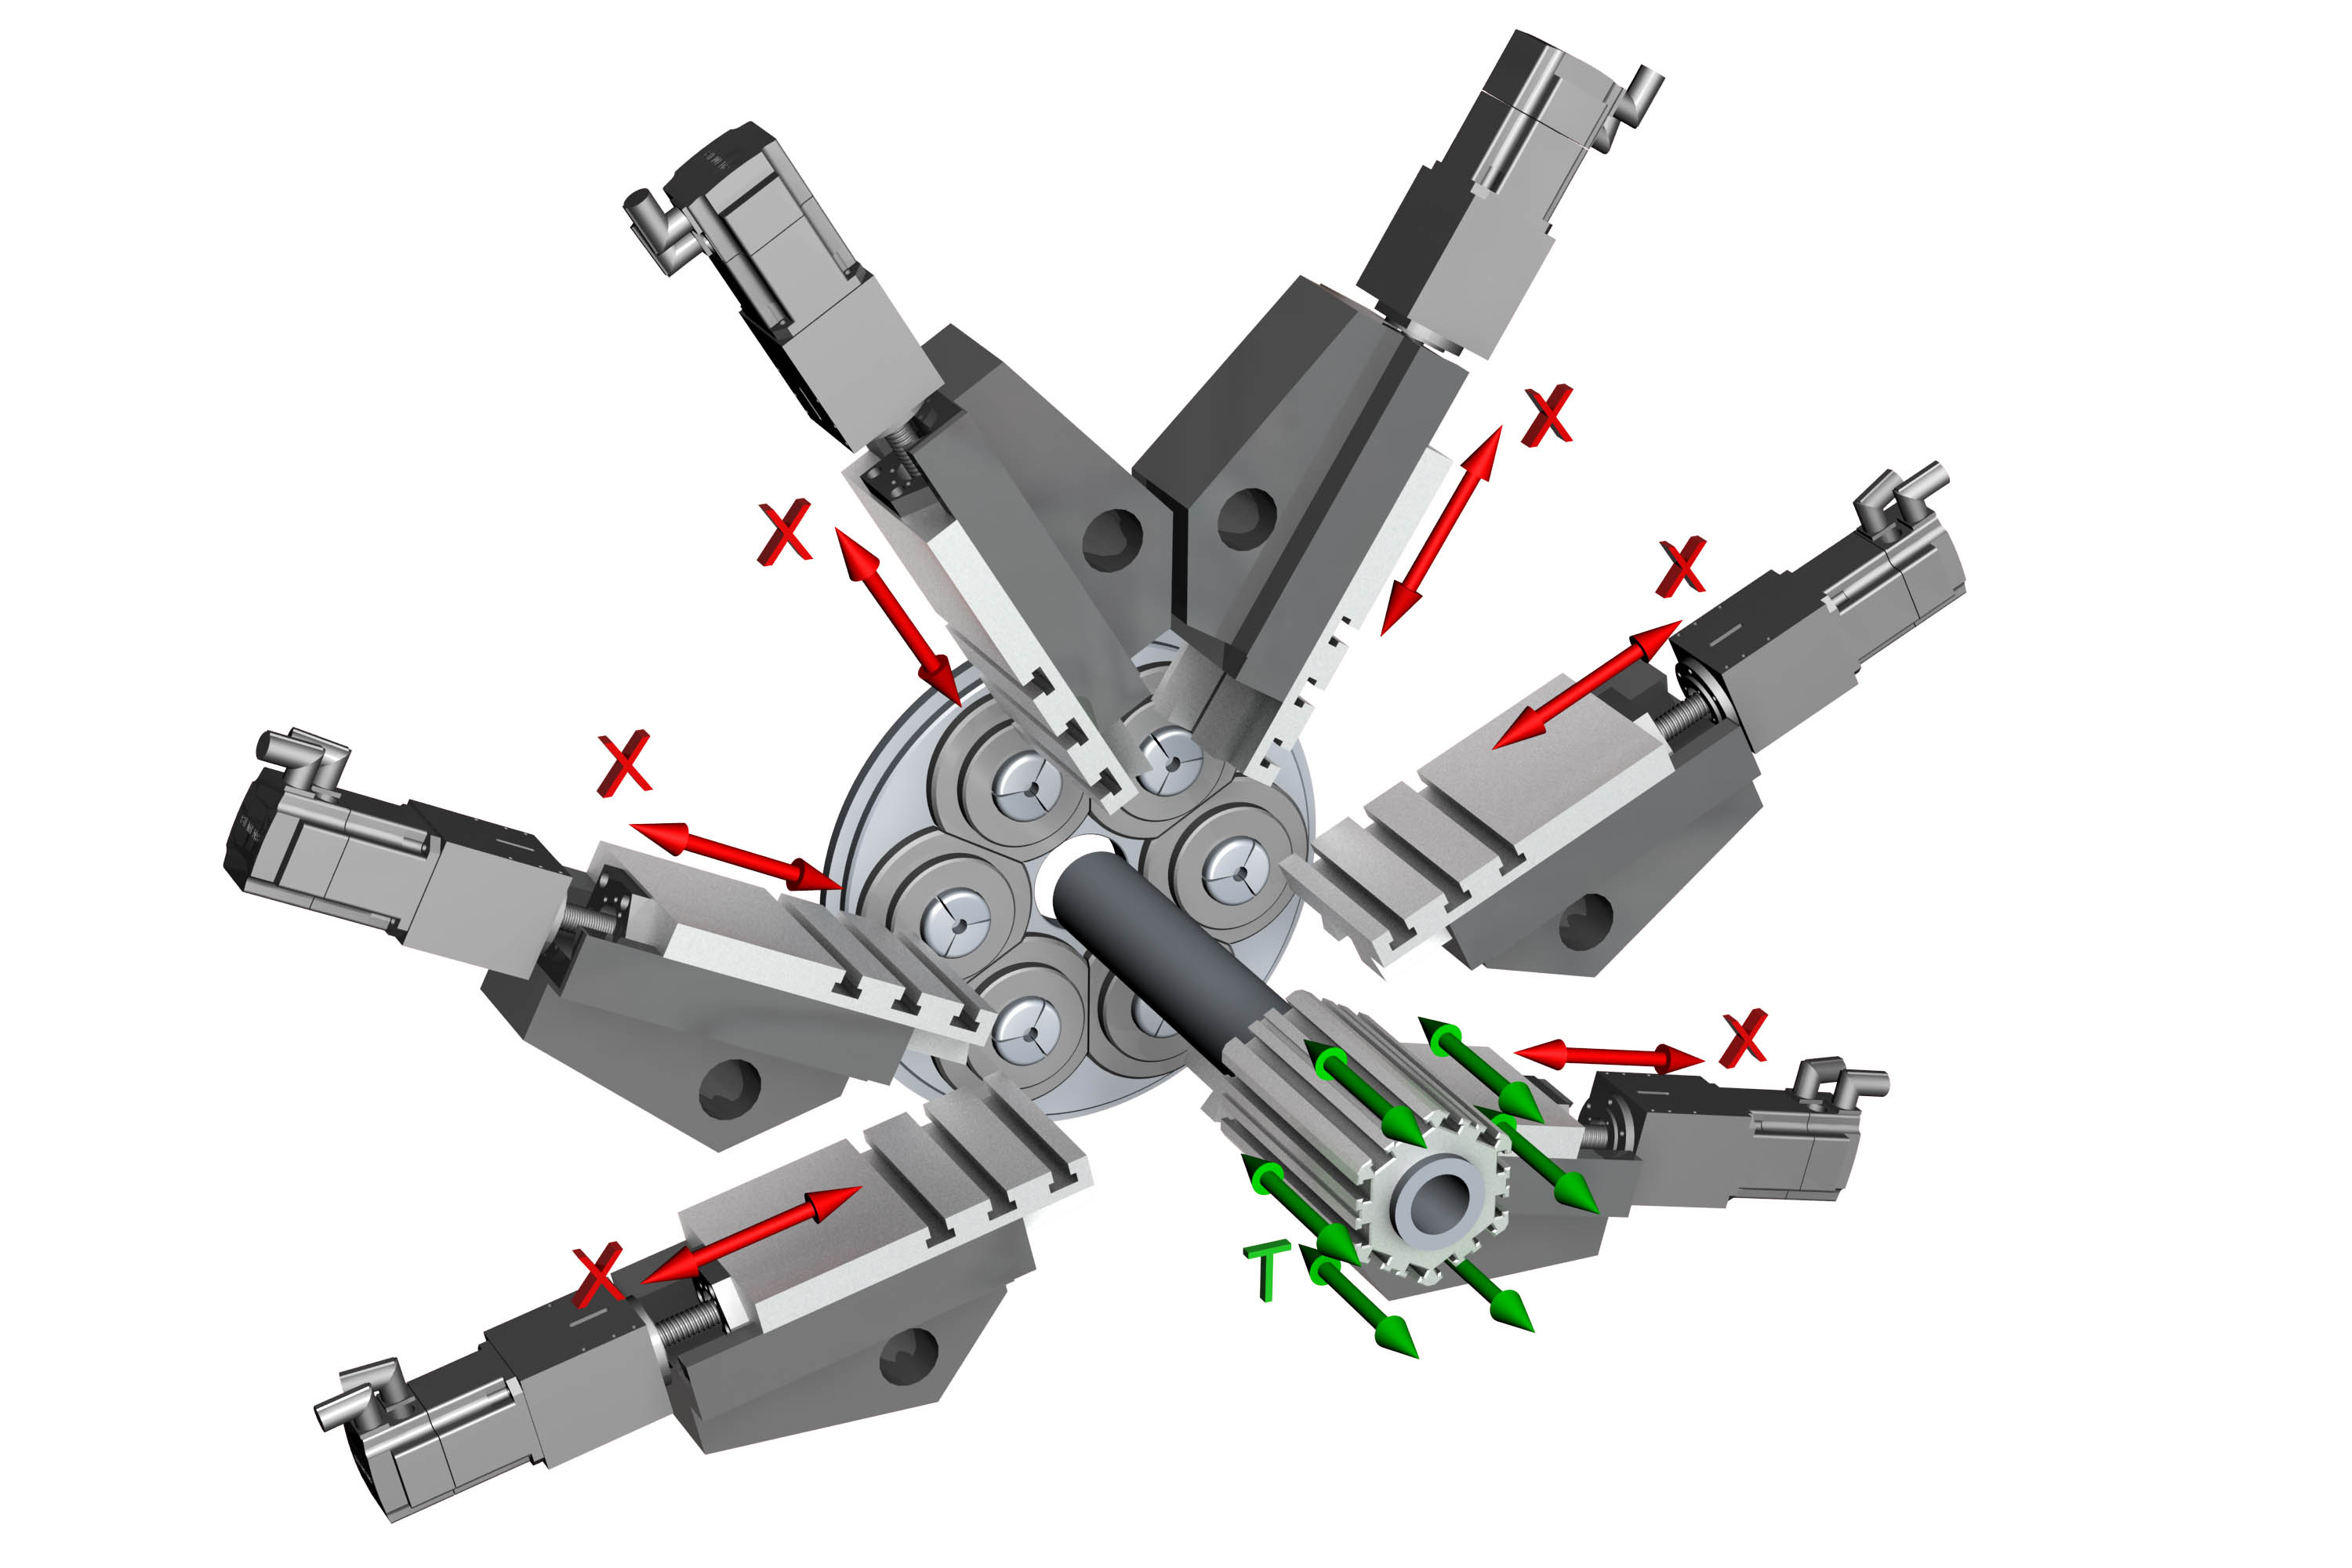
\includegraphics[width=\linewidth]{vec_vretenski_avtomat_shema.jpg}
        \caption{Shema več vretenskega avtomata
                \cite{vec_vretenska_struznica_shema}}
        \label{vec_vretenc}
    \end{center}
\end{figure}

\newpage